%%%%%%%%%%%%%%%%%%%%%%%%%%%%%%%%%%%%%%%%%%%%%%%%%%%%%%%%%%%%%
%% HEADER
%%%%%%%%%%%%%%%%%%%%%%%%%%%%%%%%%%%%%%%%%%%%%%%%%%%%%%%%%%%%%
\documentclass[preprint, authoryear]{elsarticle} % a4paper, oneside, 12pt, onecolumn
\biboptions{longnamesfirst}

%\usepackage[longnamesfirst]{natbib}
\usepackage{subfigure}
%% Math Packages %%%%%%%%%%%%%%%%%%%%%%%%%%%%%%%%%%%%%%%%%%%%
\usepackage{amsmath}
%\usepackage{amsthm}
%\usepackage{amsfonts}

\DeclareMathOperator*{\argmin}{arg\,min}


%%%%%%%%%%%%%%%%%%%%%%%%%%%%%%%%%%%%%%%%%%%%%%%%%%%%%%%%%%%%%
\begin{document}
%%%%%%%%%%%%%%%%%%%%%%%%%%%%%%%%%%%%%%%%%%%%%%%%%%%%%%%%%%%%%
\title{Stochastic Search for a Target on a Textured Background}
\author[abdn]{A. D. F. Clarke}
\ead{a.clarke@abdn.ac.uk}
\author[hw]{P. R. Green}
\author[hw]{M. J. Chantler}
\author[abdn]{A. R. Hunt}
%\date{} %%If commented, the current date is used.
\address[abdn]{School of Psychology, King's College, University of Aberdeen, Aberdeen, United Kingdom}
\address[hw]{School of Mathematical and Computer Sciences, Heriot-Watt University, Edinburgh, United Kingdom}

\begin{abstract}
Here we compare results from both a stochastic and an optimal model to human behaviour in a challenging visual search task. Both the models rely on a target visibility map based on human performance in a separate detection task. The stochastic model randomly selects the next saccade in the sequence from empirical data, while the optimal model fixates the location that will maximise the probability of detecting the target. As with previous work, we find that the number of fixations required by human observers to locate a target on a textured background is consistent with predictions from an optimal model. However, we find that a memoryless stochastic model also matches human performance. The distributions of saccade amplitudes and directions produced by the stochastic model are more similar to human behaviour than the optimal model. We conclude that, when searching for a target in noise, humans use an essentially random strategy, which achieves near optimal behaviour due to biases in the distributions of saccades we have a tendency to make. The findings reconcile the existence of highly efficient search human performance with recent studies demonstrating clear failures of optimality in single and multiple saccade tasks.
\end{abstract}

\maketitle

%%%%%%%%%%%%%%%%%%%%%%%%%%%%%%%%%%%%%%%%%%%%%%%%%%%%%%%%%%%%%
\section{Introduction}
%%%%%%%%%%%%%%%%%%%%%%%%%%%%%%%%%%%%%%%%%%%%%%%%%%%%%%%%%%%%%
The human retina provides highly accurate and detailed central vision, but acuity diminishes rapidly with eccentricity. Eye movements shift new locations to central vision, and in doing so sequentially sample finer-grained details from locations that are likely to yield important information, presumably using some combination of peripheral visual signals, inferences based on context, and top-down strategies. Each eye movement during extended search can therefore be useful for understanding how the visual system combines and prioritises information both within each fixation and across a sequence of fixations.


Much of the research on visual search to date has formalised this general issue by focusing on questions of  \itshape feature extraction \normalfont  and of \itshape strategy\normalfont. Feature extraction includes both top-down guided search \citep{wolfe2007, zelinsky2008} and stimulus-driven (saliency) effects \citep{itti-koch2000, gao2008, itti-baldi2009}.  For the abstract and discrete search items commonly used as visual search stimuli, categorical features such as colour, orientation, shape and size are often used. Simple qualitative comparisons between the search items and the target can be used to model top-down guidance \citep{pomplun2003, rutishauser-koch2007}. For more complex stimuli, such as a target hidden in image noise or in a photograph of a natural scene, there is no discrete set of items to consider and more sophisticated image processing techniques are required \citep{rao2002, zelinsky2008, pomplun2007,  hwang2009, tavassoli2009}. In either case, the output of a feature extraction mechanism is an activation map, that is, a representation of the visual array in which peaks of activity represent the priority of locations for attention.

\par

Strategy refers to the mechanism for selecting which location to inspect next. While a number of different mechanisms have been put forward, the most commonly implemented has been the Maximum A Priori (MAP) observer. The MAP observer directs saccades to the current maximum of the activation map and a simple inhibition of return (IOR) mechanism is used to stop the model returning to previously fixated maxima. Depending on the model, a maximum will either represent a search item, or the centre of gravity of a number of search items. As most previous computational models have primarily been interested in the feature extraction stage of search, the MAP observer has often been used for simplicity \citep{itti-koch2000, rao2002, pomplun2003, rutishauser-koch2007, clarke2009, zelinsky2008}.
 
 \par

An alternative to the MAP Observer is the Ideal Observer. Here, eye movements are directed to locations that are likely to yield the most information. An example of an Ideal Observer model comes from \cite{najemnik-geisler2005}, who measured visual sensitivity to a gabor patch in varying amounts of noise across a range of eccentricities and angles from fixation. From the visual sensitivity data they could generate a model of optimal eye movement behaviour that selected as the next fixation the location that would maximize the probability of detecting the target, given the amount of background noise and the known visibility of the target at various eccentricities. The number of fixations made during search for the target by the human observers (the two authors) closely matched the optimal model. In a second study \citep{najemnik-geisler2008} they also measured the fixations generated by an optimal model and found that, when averaged over all trials, the Ideal Observer matched the human spatial distribution of fixations: both the model and human observers exhibited a preference for fixating above and below the centre of the image. The idea that eye movements during search are near-optimal is broadly consistent with studies demonstrating the speed and efficiency with which eye movements can be directed to locations in a naturalistic setting that provide the most task-relevant information. A now-classic example is the demonstration of expert cricket batsmen's ability to shift their eyes rapidly to the anticipated bounce point of the ball based on its trajectory as it leaves the bowler's hand \citep{land2000}. This is a specific example of a number of studies demonstrating that eye movements are tightly constrained by task goals, and driven to maximise task-relevant information gain (for a recent review, see \citet{hayhoe2014}). 

\par

In contrast with the notion that humans are close to optimal in search behaviour is recent evidence of sub-optimality in a very similar context. \cite{morvan2012} instructed observers to first make a single eye movement to their choice of one of three squares aligned in a row, and to then make a judgement about a dot was that could appear in either the leftmost or the rightmost square. When the squares are closely spaced, the center location is the optimal choice because the dot will be visible whether it appears in the left or the right location. As the distance between the squares increases, a point is reached where the center location is no longer optimal; instead observers can maximize accuracy by selecting either the left or right location. A single saccade in this experiment represents a very similar decision to each saccade in the search task of  \cite{najemnik-geisler2005}, in that observers must use knowledge about their own visual acuity to guide their eyes to the location that is likely to yield the most information. Nonetheless, observers in Morven and Maloney's experiment were far from optimal: not only did observers not change strategy at an optimal spacing, they did not adapt their strategy to changes in the spacing of the squares at all, even though observers were given a monetary reward for each correct response. A similar conclusion was reached by \cite{verghese2012}, who demonstrated that observers failed adapt their visual search strategies to take target probability information into account, and by \cite{zhang2012} who found sub-optimal eye-hand coordination in a reaching task.
\par
How can these demonstrations of sub-optimal eye movement behaviour be resolved with \cite{najemnik-geisler2005,najemnik-geisler2008}? It is unlikely that observers would be sub-optimal at the level of a single saccade but optimal across multiple saccades. \cite{morvan2012} suggest that observers may adopt heuristics during search that generate sequences of saccades that appear optimal, but are not actually based on a fixation-by-fixation computation of posterior probability of target location. General tendencies observed in search scan-paths that have been taken to be indicative of optimal behaviour may instead be biases in saccade selection related to the scene statistics, the location of the eyes within the scene boundaries, and local mechanisms like inhibition of return and saccadic momentum. For example, \cite{over2007} have shown that search scan-paths exhibit coarse-to-fine structures, that is, observers make shorter saccades as search progresses. \cite{over2003} found that saccade directions are influenced by the edges of the search image and reported a preference for making saccades parallel to the boundaries of the stimuli.  \cite{gilchrist-harvey2006} argue that the presence of a horizontal bias in saccade directions indicates systematic scanning in visual search. They suggest these systematic tendencies can be hard to detect in scan-paths because of interactions with salience-based object selection. 
\par
Chance has also been demonstrated to play a significant role in visual search performance. Using saccade amplitude distributions \cite{motter-holsapple2001} calculated the probability of fixating the target by chance under different conditions. While this chance component decreases as the number of distracters increase, it continues to account for a sizeable fraction of performance. Random walks have been successfully used to model an observer's speed and accuracy in present/absent forced choice experiments \citep{stone1960, reeves2005}. Rather than model the spatial distribution of fixations these models simulate the observer's decision making process. The random walk occurs between two boundaries (one for a target present response and one for target absent), and is governed by a drift and bias. 
\par
A plausible alternative to the optimal model of human search behaviour is therefore that natural search behaviour is stochastic, but constrained by both scene statistics and heuristics.  Here we directly compare the performance of a random-walk model to human eye movements during search of a textured surface  for an indentation (\cite{clarke2008}, see Figure \ref{fig:exampleStimuli} for an example). We used textured surfaces because they appear naturalistic but, unlike photographs of natural scenes, they are fully controlled and parametrised. Our stochastic model randomly selects the next saccade in the sequence from the total set of saccades made from that region of the search array. This model captures the global biases of saccade programming during search reviewed above, but, unlike the optimal model, it does not take into account previous fixations or the visibility of the target given the roughness of the surface texture. For comparison, we also implemented an optimal model, based loosely on that used by  \cite{najemnik-geisler2005}. Each fixation during search was determined based on maximising the amount of information gained about the probable target location. Information gain was dependent on visual sensitivity at different eccentricities and different amounts of surface roughness, established using a separate target detection experiment. The results demonstrate that the stochastic model and the optimal model both closely match the number of fixations required to detect the target in human data. Moreover, the scan paths produced by the stochastic model are far more similar to human search than the optimal model.

%%%%%%%%%%%%%%%%%%%%%%%%%%%%%%%%%%%%%%%%%%%%%%%%%%%%%%%%%%%%%
\section{Experiment: Visual Search for a Surface Defect}
\label{sec:surfacesearch}
%%%%%%%%%%%%%%%%%%%%%%%%%%%%%%%%%%%%%%%%%%%%%%%%%%%%%%%%%%%%%

The visual search data were taken from an experiment originally published in \citet{clarke2009}. The methods and data are described here in detail.

\subsection{Surface Stimuli}
A range of rough surfaces were generated by applying Lambert's cosine law to height maps generated by a $1/f^{\beta}$-noise process. For full technical details see \citet{clarke2008}. The surface roughness is governed by $\beta$ and a scaling factor, RMS roughness, which was kept constant, $\sigma_{RMS}=1.1$ (note that RMS roughness varied in the original study \citep{clarke2009}, but we selected only the data with RMS = 1.1, corresponding to the more difficult conditions and a stronger effect of $\beta$ on search performance). The three levels of surface roughness created by varying $\beta$ will be referred to as \texttt{smooth} ($\beta=1.70$), \texttt{medium} ($\beta=1.65$) and \texttt{rough} ($\beta=1.60$). The target was created by subtracting an ellipsoid from the three dimensional surface. The target subtended $0.66^{\circ}$ of visual angle. Examples are shown in Figure \ref{fig:exampleStimuli}. For each trial a target was positioned randomly on a circle, centred on the middle of the image, with radius $1.7^{\circ} \pm 0.7^{\circ}$, $3.8^{\circ} \pm 0.7^{\circ}$ or $5.9^{\circ} \pm 0.7^{\circ}$ visual angle. 

\begin{figure}[tb]
	\centering
		\subfigure[]{
\includegraphics[width=6cm]{fig/smoothEx.png}}
		\subfigure[]{
\includegraphics[width=6cm]{fig/roughEx.png}}
	\caption{Example stimuli. This is a $256\times 256$ pixel crop of one of the (a) \texttt{smooth} and (b) \texttt{rough} surfaces. In both cases the target is shown in the centre of the image. The stimuli used in the experiment were $1024\times 1024$ pixels in size, making the target much smaller relative to the search area than what is shown here. The slight differences in the target's shape is due to randomness in the surface at the location of the target.} 
	\label{fig:exampleStimuli}
\end{figure}

\subsection{Observers}
Seven observers, aged 18-30, participated in this experiment. All had normal or corrected-to-normal vision. Observers were given several practice trials and were informed that the target would be present in all trials and would always be an indent in the surface of the same size and shape. They were instructed to respond by pressing the space bar on the keyboard once they had found the target. No time limit was imposed on the task. Observers were told to inform the experimenter if they were having great difficulty in finding the target, in which case they were allowed to skip the trial (in practice this accounted for less than 1\% of trials). A target always present task was used as previous work \citep{clarke2008} using these stimuli shows that observers fail to find target's on rougher surfaces when they have the option of making a target absent response. s

\subsection{Set-up}
Stimulus presentation was controlled by Clearview (Tobii Technology Inc). All stimuli were $1024 \times 1024$ pixels in size and displayed on a NEC LCD2090UXi monitor. The pixel dimensions were 0.255mm by 0.255mm resulting in images with physical dimensions 26.1cm by 26.1cm. The monitor was linearly calibrated with a Gretag-MacBeth Eye-One; maximum luminance was set at 120 cd/m$^2$. This results in the rendered images appearing as if they were under bright room lighting conditions.

A Tobii x50 eye-tracker was used to record observers' gaze patterns. The fixation filter was set to count only those fixations lasting longer than 100 ms within an area of 30 pixels. The accuracy of the eye-tracker was $0.5^{\circ}$ to $–0.7^{\circ}$ and the spatial resolution was $0.35^{\circ}$. The viewing distance was controlled by use of a chin rest placed 87cm away from the display monitor. At this distance, one pixel is approximately 1 arcminute of visual angle; images subtend $16.7^{\circ}$ and the targets subtend $0.66^{\circ}$ of visual angle. 

\subsection{Results}
\label{sec:SearchPerf}
The number of fixations required to find the target is shown in Figure \ref{fig:nFixclarke2009}. Using a generalised linear mixed model with random effects (the \texttt{lme4} package for \texttt{R}, \texttt{family="poisson"}) we confirm that both roughness ($\beta$) and target eccentricity, along with their interaction, have a statistically significant effect ($\alpha=0.05$) on the number of fixations required to detect the target. Saccade summary statistics are shown in Figure \ref{fig:saccsummclarke2009} and are similar to those reported in other studies. 

\begin{figure}
	\centering
		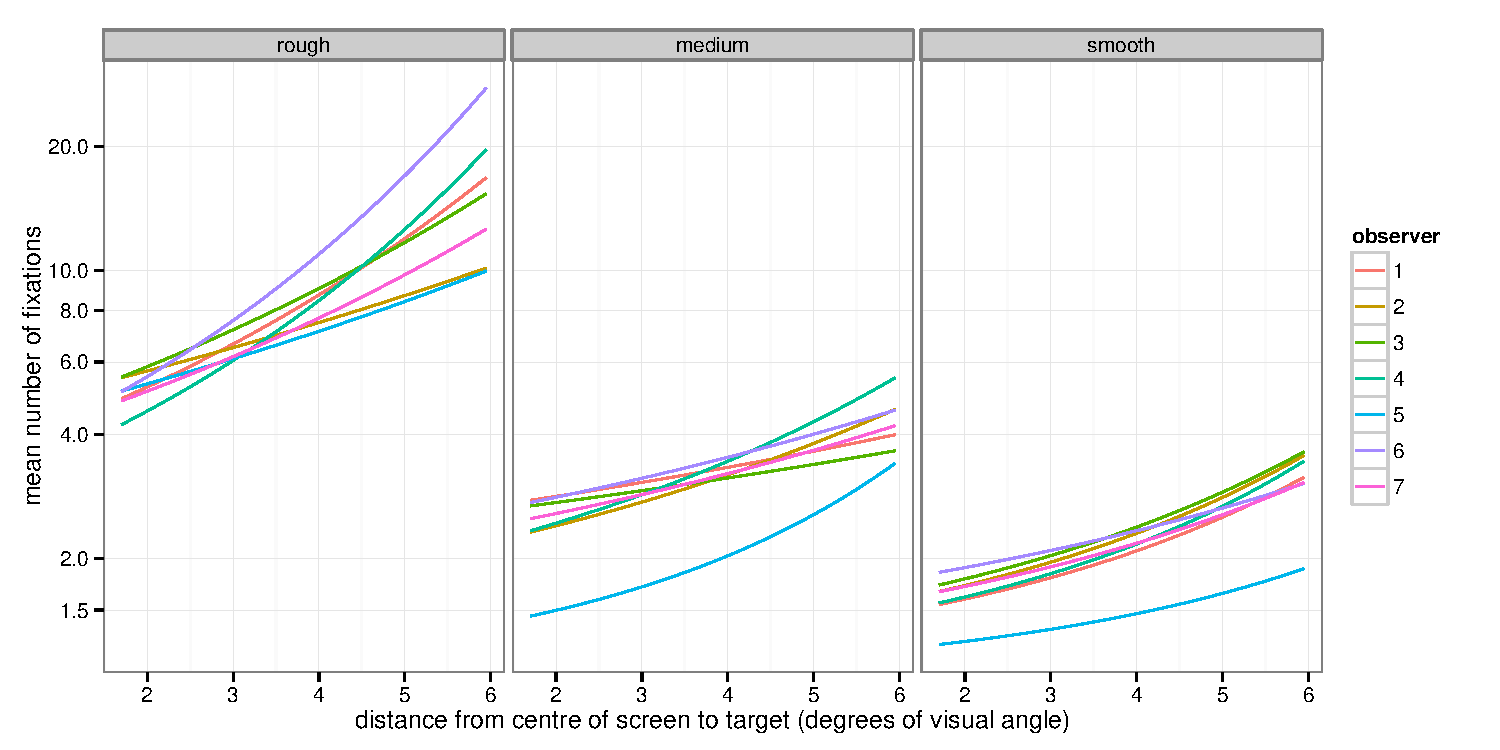
\includegraphics[width=12cm]{fig/numFixObs.pdf}
	\caption{Performance for each of the seven observers for each of the three conditions to illustrate the systematic variation between conditions. Only the model fits are shown here to reduce clutter. Boxplots showing the distribution of the number of fixations required to find the target are shown for each observer in Figure \ref{fig:numFixHumanModel}}
	\label{fig:nFixclarke2009}
\end{figure}

\begin{figure}
	\centering
		\subfigure[]{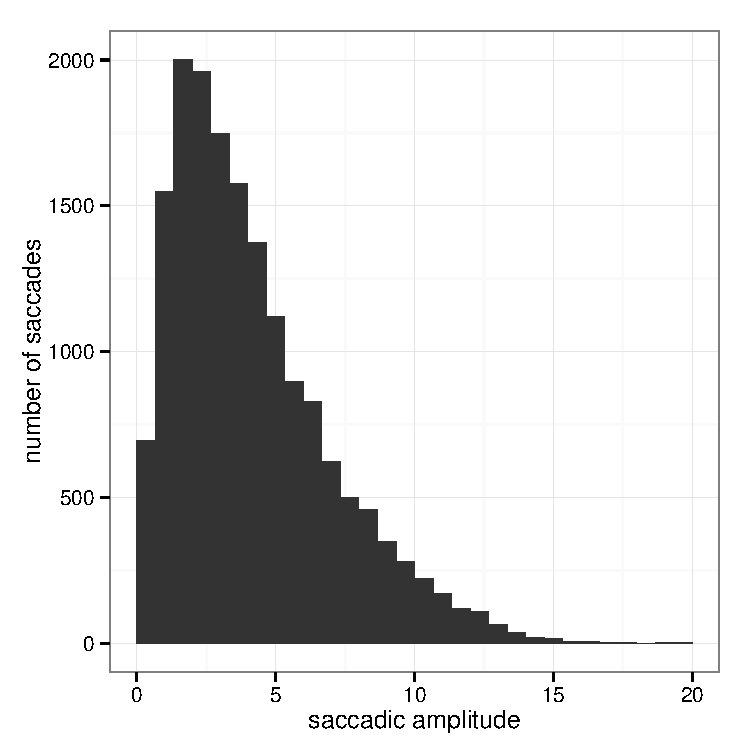
\includegraphics[width=6cm]{fig/saccAmp.pdf}}
		\subfigure[]{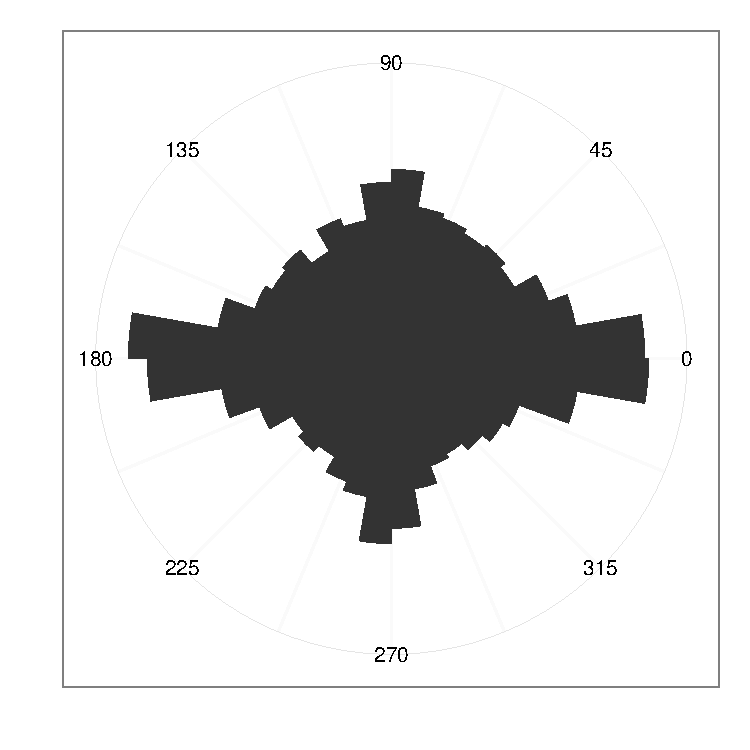
\includegraphics[width=6cm]{fig/roseplot.pdf}}
	\caption{Summary saccade statistics over all observers and all conditions. (a) shows the histogram of saccade amplitudes, while (b) shows the distribution of saccade directions. }
	\label{fig:saccsummclarke2009}
\end{figure}

%%%%%%%%%%%%%%%%%%%%%%%%%%%%%%%%%%%%%%%%%%%%%%%%%%%%%%%%%%%%%
\section{Target detection experiment}
\label{surfacesearchdetectprob}
%%%%%%%%%%%%%%%%%%%%%%%%%%%%%%%%%%%%%%%%%%%%%%%%%%%%%%%%%%%%%

Both the stochastic and optimal search models make use of a target visibility map that specifies the probability of the target being detected from a given fixation point.  Here we outline the experiment used to empirically obtain the target detection function used in the models. The goal was to match as closely as possible the detection task observers would need to perform during each fixation during search. We therefore made the target location uncertain (unlike in \cite{najemnik-geisler2005,najemnik-geisler2008}, in which the target location was cued on every trial).

\subsection{Stimuli}

Surface textures were created as detailed above. For the target present trials, the target was located at one of 72 potential locations: nine different eccentricities were used $0.84^{\circ}\leq r\leq 7.5^{\circ}$, and eight evenly spaced orientations. For each parameter combination, 20 different trials were created; by changing the random seed used to create the noise we can create textured surfaces on each trial that are unique but statistically identical. Because the target is difficult or impossible to detect at larger eccentricities, we balanced this by using fewer target absent trials so that the target would be apparently present on about half of trials. Based on pilot results, we created 160 target absent trials for each value of $\beta$, giving a total of 2160 target present trials and 480 target absent trials. This ratio of target present to absent trials ensured that observers made roughly equal numbers of ``present'' and ``absent'' responses.

\subsection{Observers}

Two observers carried out all the trials, split into twenty blocks of 132 trials, over a number of days. They were paid \pounds50 each. They were instructed to keep their eyes fixated on the centre of the image. After each trial, they were asked to respond with a button press to indicate if they had seen the target or not. The research was conducted in accord with the Code of Ethics of the World Medical Association (Declaration of Helsinki) and informed consent was obtained for both observers. 

\subsection{Set-up}

 Each trial consisted of a fixation cross (500ms), stimulus (200ms), white noise mask (500ms), and finally a fixation cross was displayed until a target present or absent response was given. 
\par
A Tobii x50 eyetracker was used to sample the observers' gaze every 20ms and trials were included in the further analysis only if (i) the mean gaze location was within $1^{\circ}$ of the central fixation cross (ii) the standard deviation of the gaze's $x$ and $y$ components was less than $2/3^{\circ}$.

\subsection{Results}

$13.6\%$ of trials were removed from analysis (due to breaking central fixation). We first checked the false positive rate on target absent trials, Table \ref{tab:falsepostives}, and find that it is very low in all cases. We can therefore focus on the probability of detecting the target when it was present as a measure of visibility. While this means we are potentially over-estimating the probability of finding the target, this will bias both the stochastic and optimal models in the same way.

\begin{table}
\centering
\begin{tabular}{c|ccc}
$\beta$	& rough & medium & smooth \\
\hline
observer 1 	& 0.028 & 0.020 & 0.007 \\
observer 2	& 0.090 & 0.029 & 0.015 \\
\end{tabular}
\caption{The proportion of false positives is less than 0.1 in all conditions.}
\label{tab:falsepostives}
\end{table}

\begin{table}
\centering
\begin{tabular}{c|ccc}
$\beta$	& rough & medium & smooth \\
\hline
$b_1$ 	& 0.16 & 1.78 & 2.92 \\
$b_2$	& -0.50 & -0.73 & -0.75 \\
$b_3$	& 0.004 & 0.032 & 0.020 \\
\end{tabular}
\caption{Coefficients used in Equation \ref{eq:targDet}, the target detection function.}
\label{tab:targdetcoef}
\end{table}

As both observers' results are similar, we collapse over observer and fit a generalised linear model (\texttt{family="binomial"} with \texttt{response $\sim$ beta * (r + x2)} where $r$ is distance from fixation to target, and $\texttt{x2}=x^2$. The resulting target detection functions are shown in Figure \ref{fig:targDet}. The following are statistically significant: $\beta$  ($\chi^2(2)=394$, $p<0.001$), $r$, ($\chi^2(1)=632$, $p<0.001$), $x^2$, ($\chi^2(1)=17$, $p<0.001$), and the interaction between $\beta$ and $r$ ($\chi^2(2)=10$, $p=0.006$). Model coefficents are showin in Table \ref{tab:targdetcoef}. 

%\begin{figure}
%	\centering
%	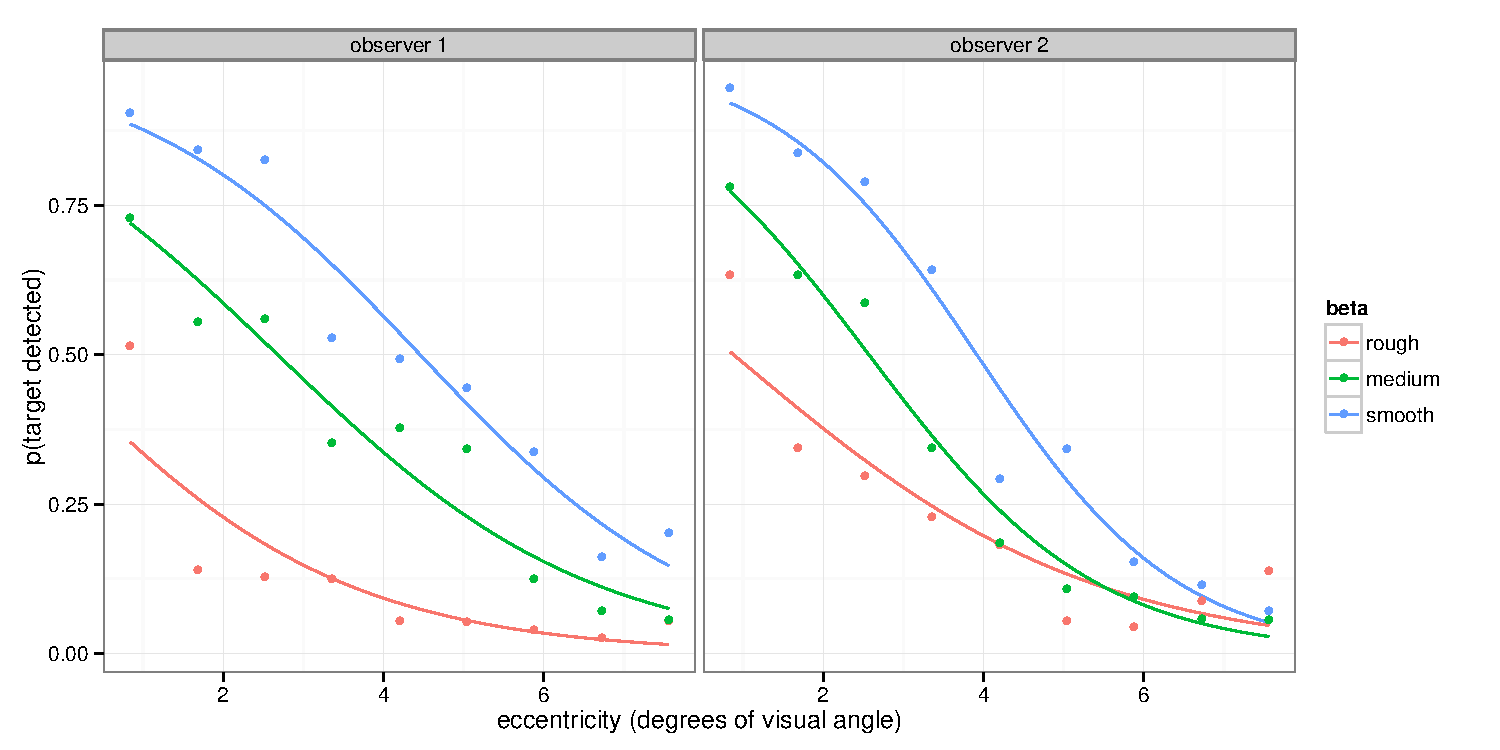
\includegraphics[width=12cm]{fig/targDetModelEccOnly.pdf}
%	\caption{Target detection probability for the two observers, collapsed over the angle of the target in polar coordinates. The lines show a logistic regression model fit to the data.} %what is phi?
%	\label{fig:targDetCollapsedPhi}
%\end{figure}

\begin{figure}
	\centering
	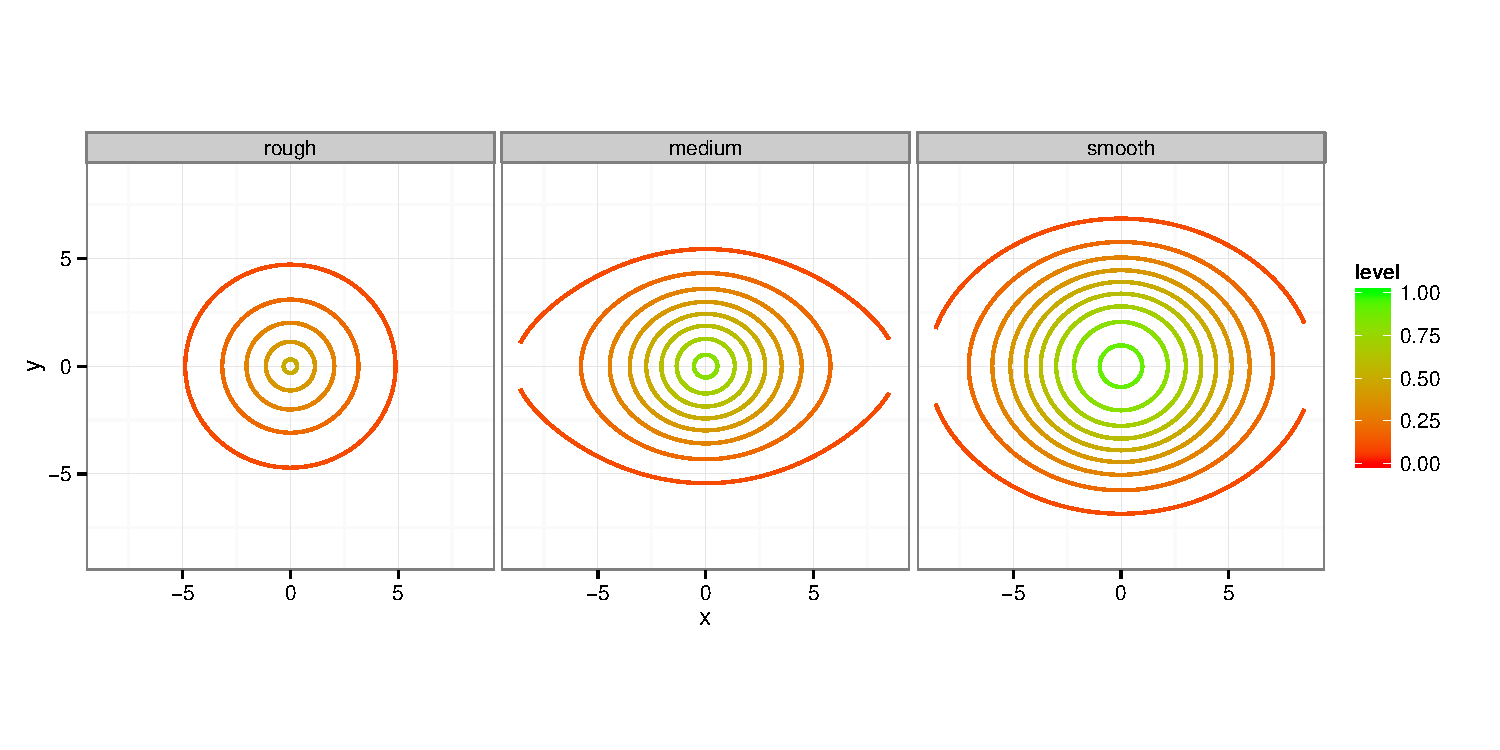
\includegraphics[width=12cm]{fig/targDetResults.pdf}
	\caption{Target detection model. Notice that in the \texttt{rough} condition, the the target is frequently not detected even when presented at fixation}. 
	\label{fig:targDet}
\end{figure}


%%%%%%%%%%%%%%%%%%%%%%%%%%%%%%%%%%%%%%%%%%%%%%%%%%%%%%%%%%%%%
\section{Search Strategies}
%%%%%%%%%%%%%%%%%%%%%%%%%%%%%%%%%%%%%%%%%%%%%%%%%%%%%%%%%%%%%

Here we describe two different models - stochastic and optimal search - of the search task described in Section \ref{sec:surfacesearch}. Both models are based on the visibility map derived in Section \ref{surfacesearchdetectprob}. That is, the probability of detecting a target located at $(x,y)$ is given by

\begin{equation}
 p(d_{x,y}|f_i,\beta) = F(\vec{b_1}\cdot\vec{\beta} + \vec{b_2}\vec{\beta} r + \vec{b_2}\vec{\beta}x^2)
 \label{eq:targDet}
\end{equation} 

where $\vec{\beta}$ is a vector encoding the categorical factor $\beta$ and $F$ is the logistic transform:
\begin{equation}
F(z)= \frac{1}{1+e^{-z}}
\end{equation}

The coefficients are given in Table \ref{tab:targdetcoef} and this function is illustrated in Figure \ref{fig:targDet}.

\subsection{Stochastic Searcher}

For each fixation, the stochastic searcher uses the target detection function given in Equation \ref{eq:targDet} to determine if the target is present. To decide where to fixate next, this model samples a saccade at random (from empirical data), conditioned on the current fixation location, $S(x',y',x_i, y_i)=p\left((x',y')|(x_i,y_i)\right)$. We base $S$ on the distribution of saccades recorded in Section \ref{sec:surfacesearch}, Figure \ref{fig:saccsummclarke2009}. To estimate $S$, we start by quantising the fixations to a $Q\times Q$ grid ($Q=32$). Then we simply count the number of saccades from $(q_{x_1}, p_{y_1})$ to $(q_{x_2}, p_{y_2})$, $1\leq x_i, y_i \leq Q$. As the last saccade in each trial is likely to be directed towards the target, rather than searching for the target, these saccades are not included in this distribution. We then convolve $S$ with a four-dimensional Gaussian filter ($\sigma=3$). Figure \ref{fig:saccDistExample} shows a simplified version of this distribution (with $Q=3$). 

\begin{figure}
	\centering
	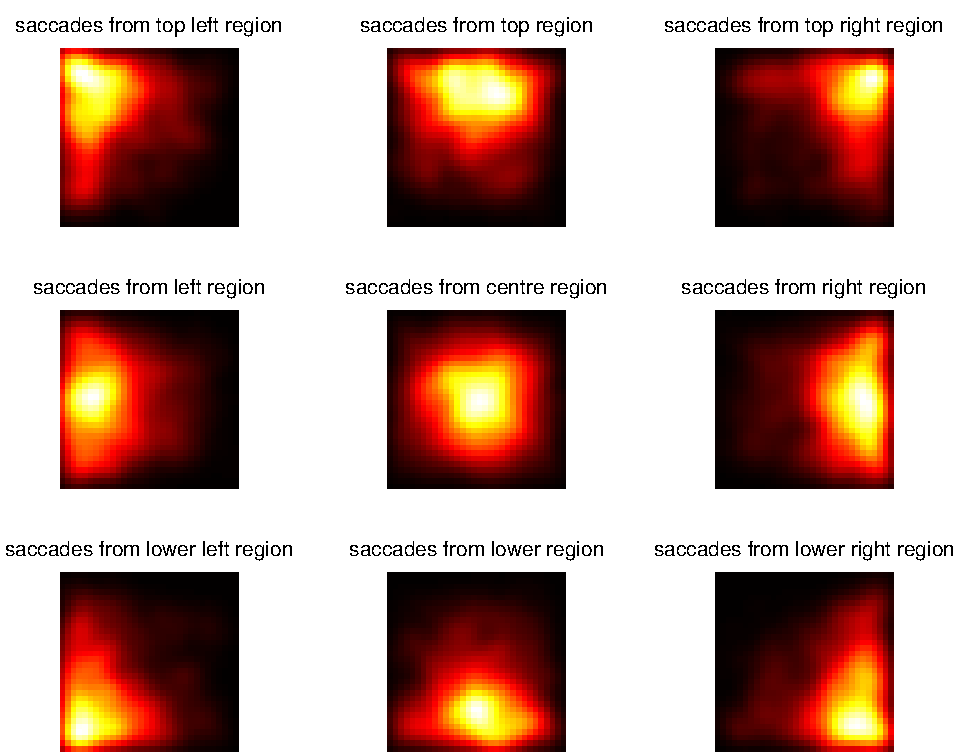
\includegraphics[width=10cm]{fig/saccDistExample.pdf}
	\caption{Each subplot shows a hotspot map of fixation locations from a different region of the stimuli. For example, we can see that saccades originating from the corner regions tend to be directed back towards the centre, or along one of the edges.}. 
	\label{fig:saccDistExample}
\end{figure}

The use of this distribution allows the stochastic searcher to act as a realistic baseline: it will make saccades with amplitudes and directions similar to those made by human observers, and it avoids making saccades to locations outside of the search area. On the other hand, as the probability of making a fixation to a given location is only conditioned on the sample of saccades to that region in previous data, it has no memory of where it has looked before, and it has no notion of inhibition of return or saccadic momentum. Furthermore, the stochastic searcher does not adjust its behaviour based on the difficulty of the search task or the probability of detecting the target. 

\subsection{Optimal searcher}

The optimal model uses the target detection function, $p(d_{x,y}|f_i,\beta)$, to estimate $p(t_{x,y})$, the probability that the target is located at $(x,y)$, defined as:

\begin{equation}
P_i(x,y) = p(t_{x,y} | \beta, f_1,\ldots, f_i)
\end{equation}

\subsubsection{Probability that target is located at $(x,y)$}

We start off by setting $P_0$ to our prior on where the target is likely to be located. We will use a uniform distribution over the search area: $P_0(x,y) \propto \hat{P_0}=1$. (i.e.,  $P_0(x,y) = \frac{1}{N^2}$, where $N^2$ gives the area of the search stimulus). However, $P_0$ could be set to any arbitrary distribution. 

After each fixation, we use Equation \ref{eq:targDet} to check if the target has been detected. If the target is detected then $P_i = 1$ at the target's location, 0 everywhere else and the search process is terminated. If the target is not detected then, assuming (i) perfect memory and (ii) that $p(d_{x,y} | \beta, f_i)$ $\forall i$ are independent, we define $P_i\propto \hat{P_i}$ as: 

\begin{align}
P_i(x,y) \propto \hat{P}_i(x,y)	&= p(t_{x,y} | \beta, f_1,\ldots, f_i)\\
 							&= p(t_{x,y} | \beta, f_1,\ldots, f_{i-1})\times p(t_{x,y} | \beta, f_i)\\
 							&= \hat{P}_{i-1}(x,y)\times (p(\neg d_{x,y} | \beta, f_i))
 			\label{eq:Pupdaterule}
\end{align}

The logic of this is as follows. Consider our first fixation $f_1 = (x_1,y_1)$, a potential target location $(x',y')$ close to the current fixation, and let us assume that we have not yet detected the target. If the target was located at $(x',y')$, then we would have a relatively good chance of detecting it. For the purpose of this explanation, let us assume that $p(d_{x',y'}|f_1)=0.8$, that is, if we fixate at $(x_1,y_1)$ then we have a $80\%$ chance of detecting the target if it is located at $(x',y')$. Now let us consider the probability that the target is indeed located at $(x',y')$. If there were an $80\%$ chance of target detection, but no target was detected, there is (up to a normalisation step to take into account the total number of possible target locations) a $20\%$ chance that the target is located at $(x',y')$. More generally:
\begin{equation}
p(t_{x',y'}|f_1) \propto p(\neg d_{x',y'}|f_1)
\end{equation}
We can iterate over successive fixations using Equation \ref{eq:Pupdaterule}.

\subsubsection{Choosing where to fixate next}

Once we have calculated $\hat{P}_i$ we use it to select the next fixation location. As we are only calculating $P_i$ up to a normalisation constant, the map that we actually calculate, $\hat{P_i} =  \hat{P}_{i-1}(x,y)\times p(\neg d_{x,y} | \beta, f_i)$, has the property that $\hat{P}_i(x,y)\leq\hat{P}_{i-1}(x,y)$ $\forall i,x,y$. This can be thought of as measuring how much we still have to search different regions of the stimulus. Our model will make a fixation at the point $f_{i+1}=(x_{i+1},y_{i+1})$ that maximises the difference between $P_i$ and $P_{i+1}$. This can be expressed as: 

\begin{equation}
(x_{i+1},y_{i+1}) = \argmin_{f_j=(x_j,y_j)}\sum_{x,y} P_i(x,y)p(\neg d_{x,y}|\beta, f_j)
\end{equation}

This process is illustrated in Figure \ref{fig:planningFix}. In order to reduce computation time, the simulation takes place at a lower resolution, with $N=256$ rather than 1024.


\begin{figure}[tb]
	\begin{center}
		\subfigure[fixation 1]{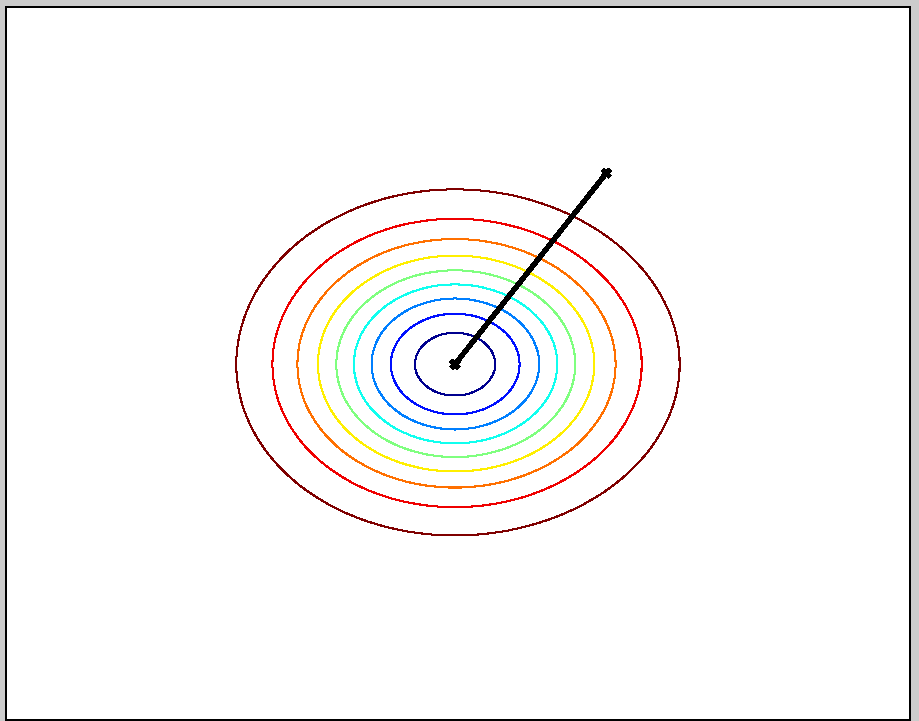
\includegraphics[width=3cm]{fig/fixplanning/fixation1.pdf}}
		\subfigure[fixation 2]{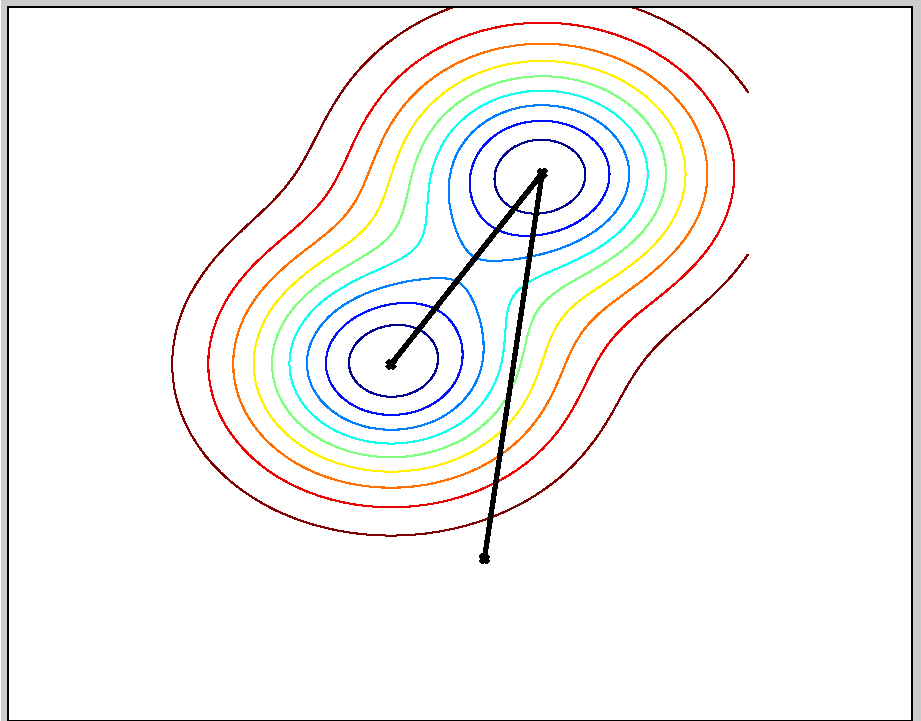
\includegraphics[width=3cm]{fig/fixplanning/fixation2.pdf}}
		\subfigure[fixation 5]{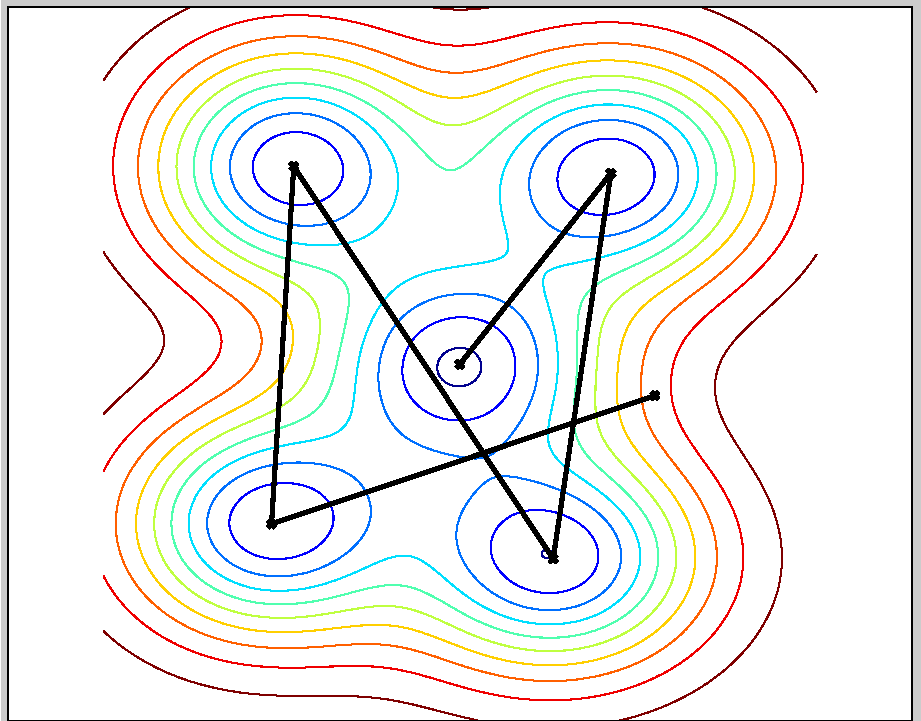
\includegraphics[width=3cm]{fig/fixplanning/fixation5.pdf}}
		%\subfigure[fix 10 $\beta=1.6$]{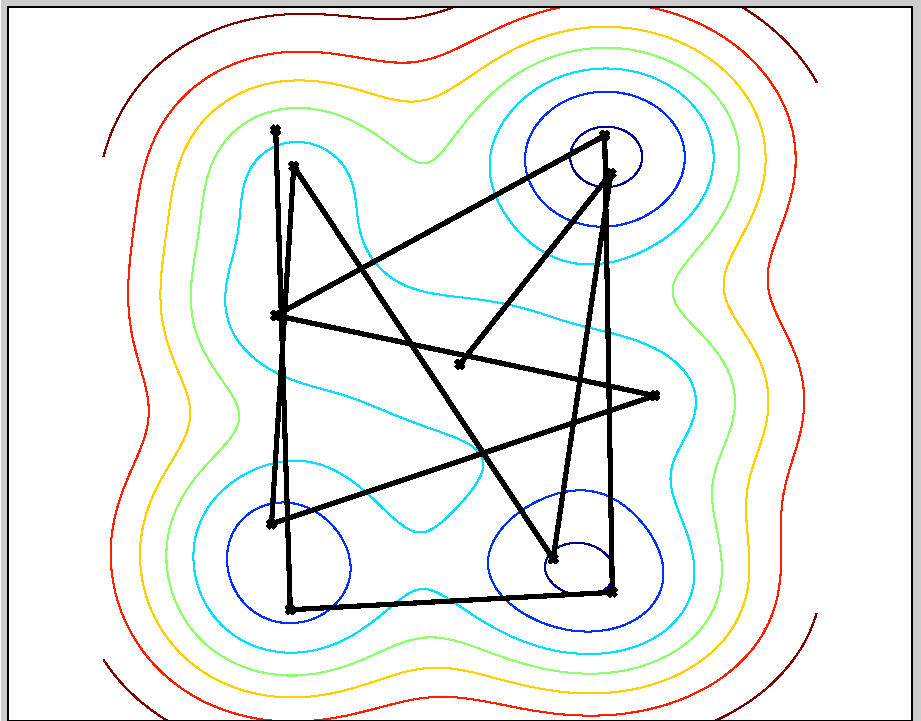
\includegraphics[width=3cm]{fig/fixplanning/fixation10.pdf}}
		\subfigure[fixation 1]{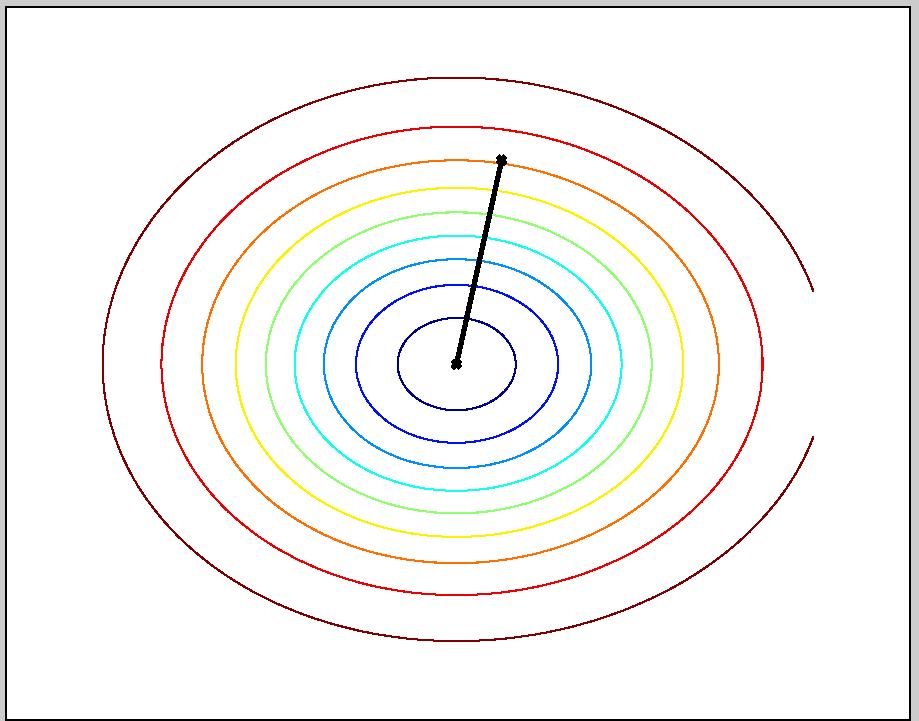
\includegraphics[width=3cm]{fig/fixplanning/fixation1-2.pdf}}
		\subfigure[fixation 2]{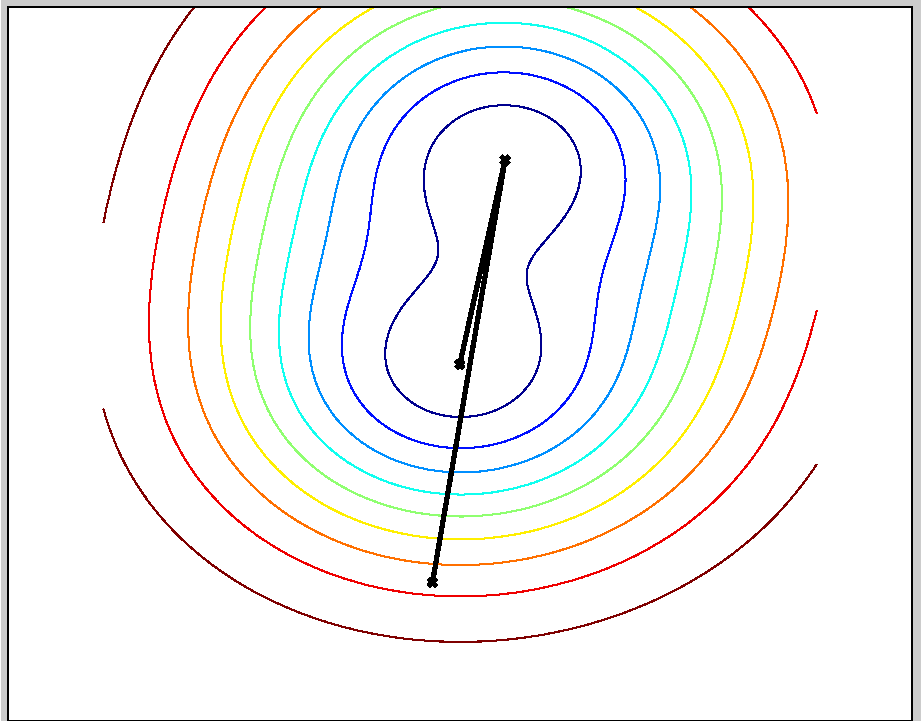
\includegraphics[width=3cm]{fig/fixplanning/fixation2-2.pdf}}
		\subfigure[fixation 5]{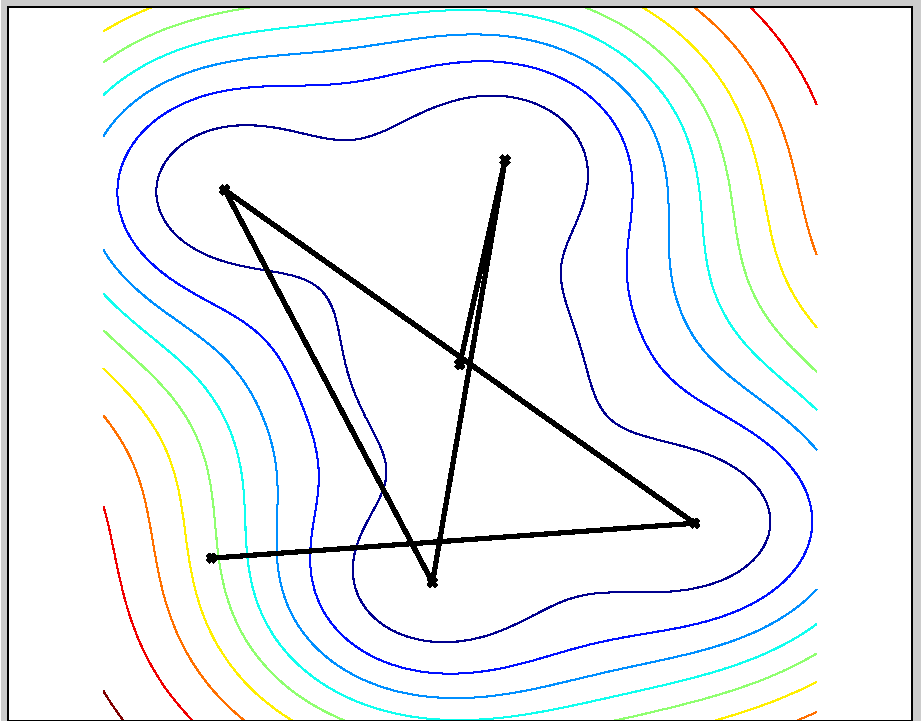
\includegraphics[width=3cm]{fig/fixplanning/fixation5-2.pdf}}
		%\subfigure[fix 10 $\beta=1.7$]{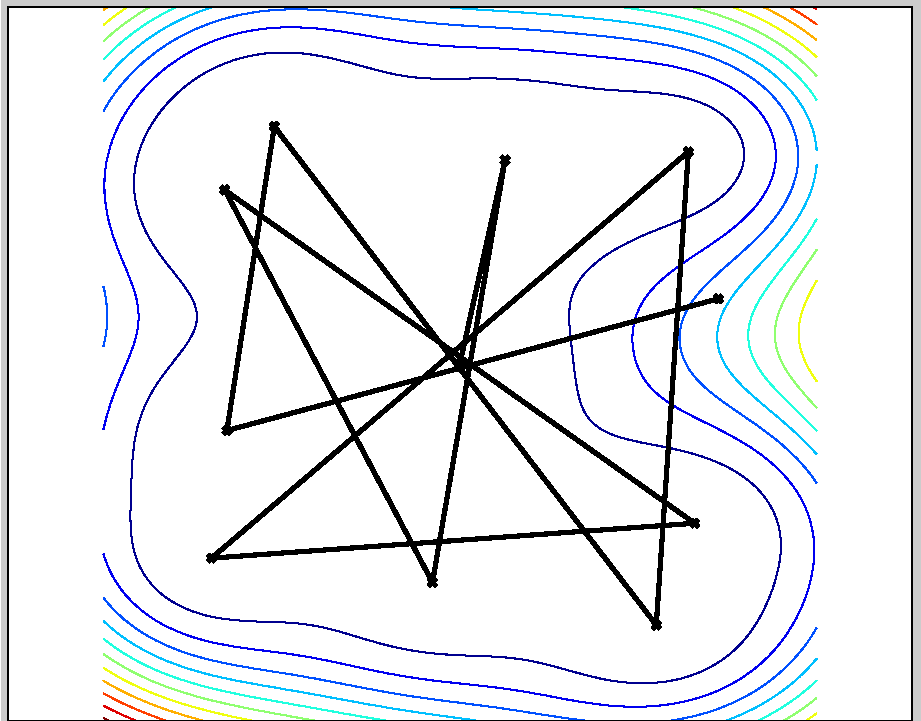
\includegraphics[width=3cm]{fig/fixplanning/fixation10-2.pdf}}		
	\end{center}
	\caption{This figure shows how $P_i$ is updated with each fixation and used to plan the next fixation. (a), (b) and (c) show fixation 1,2, and 5 in the hard condition, while (d), (e) and (f) show how search progresses in the easy condition.}
	\label{fig:planningFix}
\end{figure}

\section{Comparing human observer to the models}

We now compare the two models to human performance, as detailed in Section \ref{sec:SearchPerf} by simulating search over the same number as trials as used in the original experiment. In agreement with \citet{najemnik-geisler2008}, we find that, in terms of the number of saccades required to find the target, human performance is consistent with an optimal search strategy (Figure \ref{fig:numFixHumanModel}). However, the stochastic searcher offers very similar performance. Indeed, a one-tailed, paired $t$-test between the two models gives $t(719)=-0.737$, $p=0.23$\footnote{As one would expect, this difference becomes statistically significant if more data is generated from the simulations: with 100 trials per condition we get $t(7199)=-3.48$, $p<0.001$ However, this difference corresponds to the optimal model finding the target on average half a fixation faster than the stochastic model.}. As we can see from Figure \ref{fig:numFixHumanModel}, both models are both very similar to human fixation data in terms of the number of fixations.

\begin{figure}
	\centering
	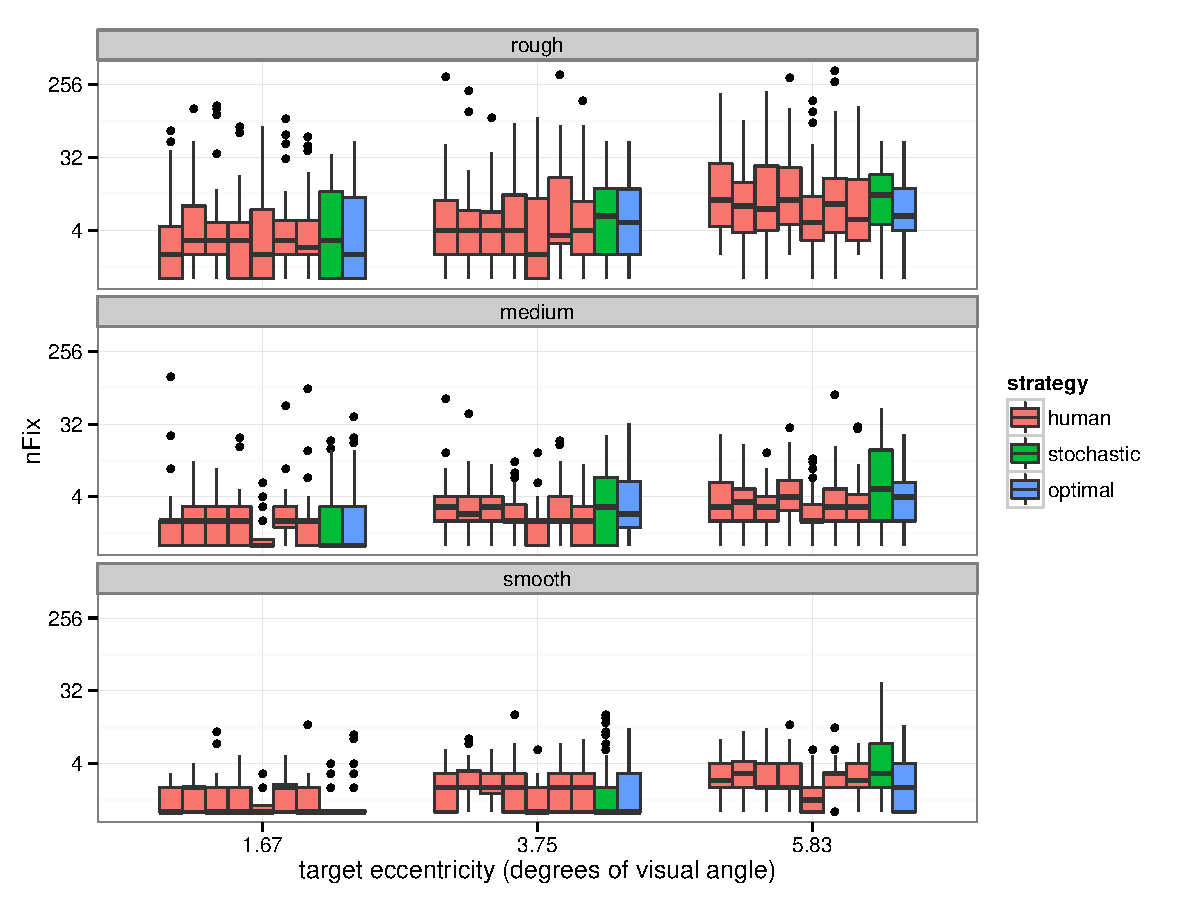
\includegraphics[width=10cm]{fig/numFixHumanModel.pdf}
	\caption{Number of saccades made by human observers and search simulations. The two models differ very little from human observers.} 
	\label{fig:numFixHumanModel}
\end{figure}

We can also look at the saccade statistics to see if they offer a way to distinguish between the two models and detemine which offers the more human-like behaviour. Figure \ref{fig:exScanpaths} shows some example scanpaths. We can see that the optimal model favours making fixations in the centres of the four quadrants of the search area. Figures \ref{fig:onetwostats} show the distributions of saccade amplitudes and directions and we can clearly see that there are large differences between the behaviour of the optimal model and human observers. 

\begin{figure}
	\centering
	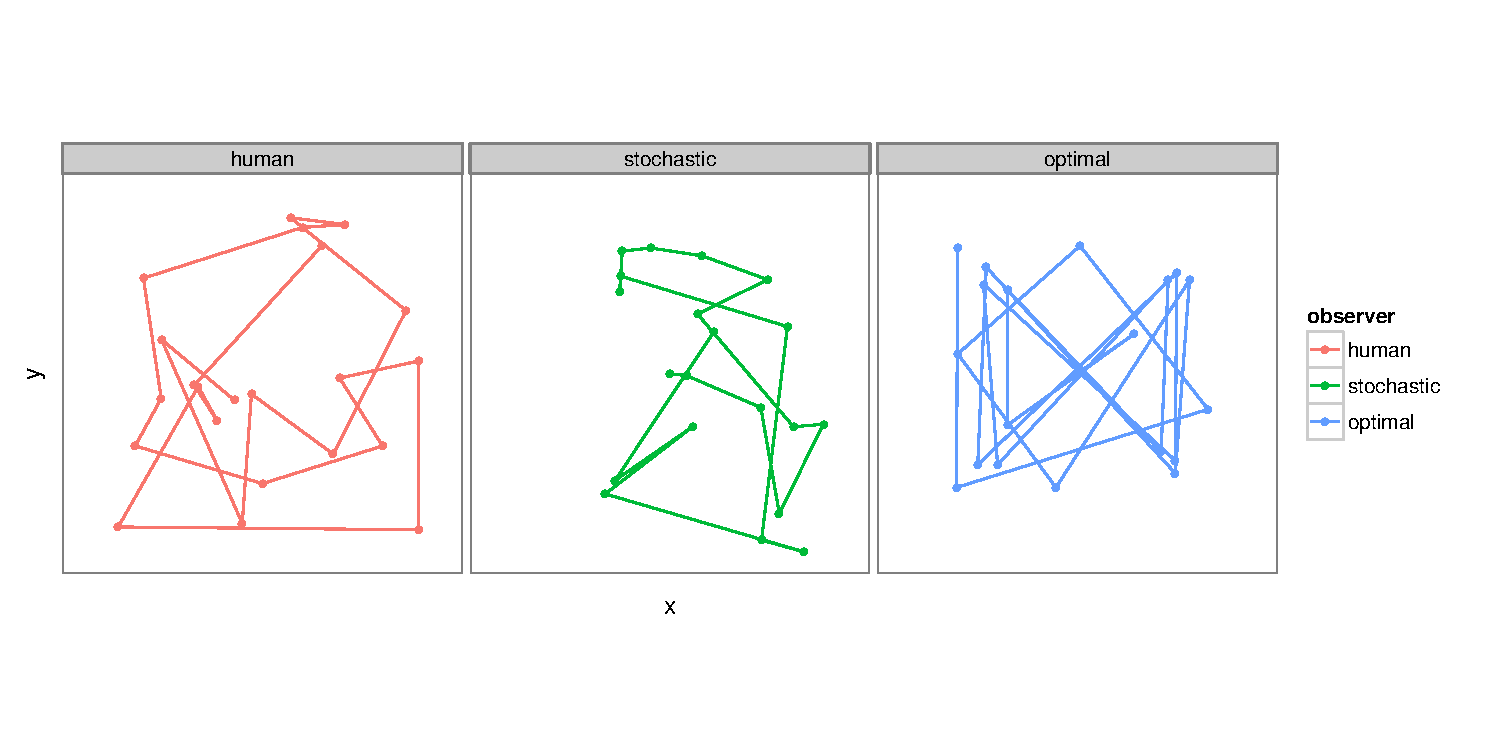
\includegraphics[width=10cm]{fig/exScanpaths.pdf}
	\caption{Example scanpaths made by a human, stochastic and optimal observer. We can see that similarly to \citet{najemnik-geisler2008}, the optimal model shows a preference for several fixed points on the sitmulus. These are the locations which maximise the information gained via para-foveal vision, and minimise the proportion of the effective field of vision that falls outside of the search area. The centre is avoided after the initial fixation because it is frequently sampled by peripheral vision.} 
	\label{fig:exScanpaths}
\end{figure}


\begin{figure}
	\centering
	\subfigure[]{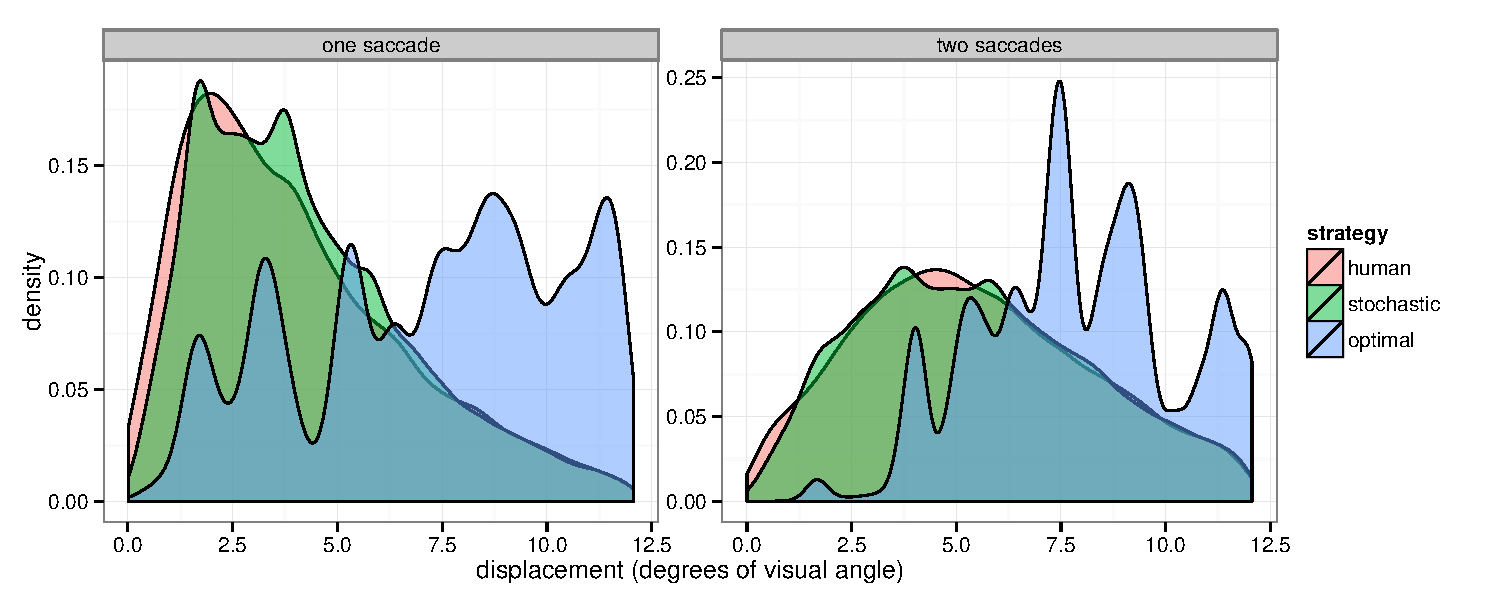
\includegraphics[width=10cm]{fig/onetwosaccamp.pdf}}
	\subfigure[]{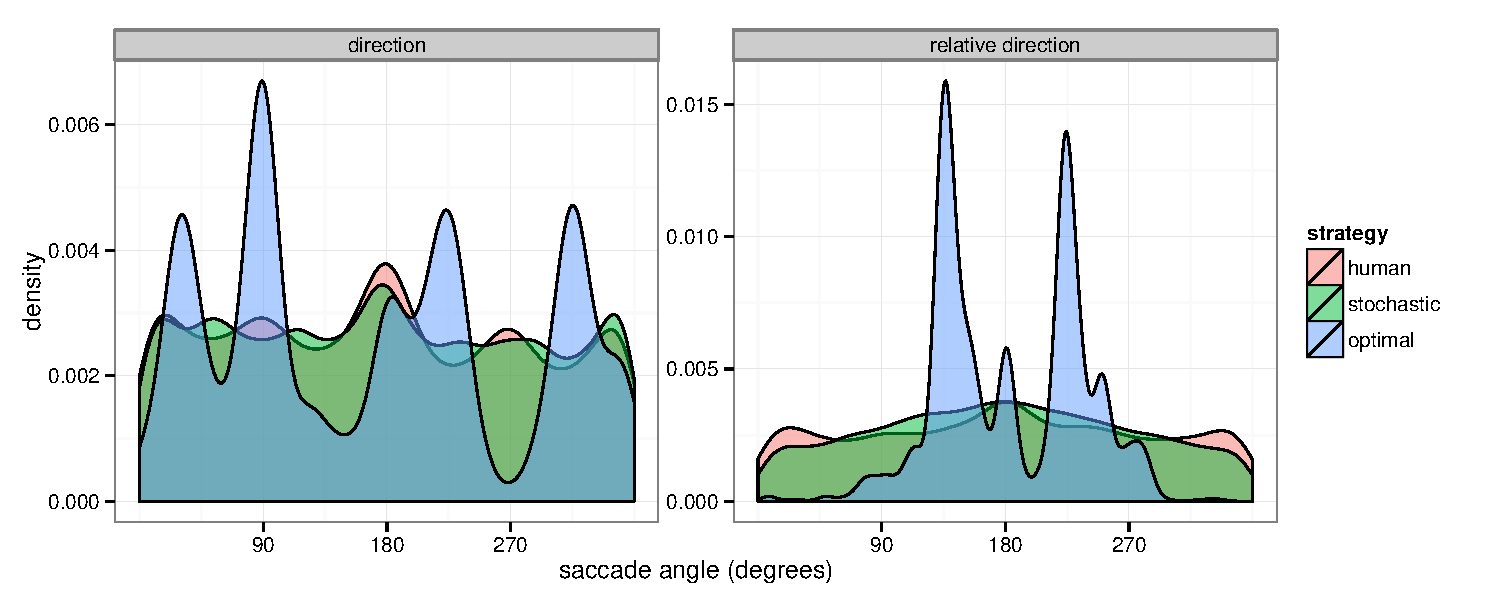
\includegraphics[width=10cm]{fig/saccAngles.pdf}}
	\caption{(a) Displacement over one and two saccades. (b) Absolute and relative direction of saccades.The fact that the stochastic model matches the distribution of displacement and direction over a single saccade is a direct result of sampling from empirical data and is therefore unsurprising. The distributions over two saccades are, however, more interesting because human observers might be expected to be biased away from repetition of fixations more than stochastic sampling would predict.}
	\label{fig:onetwostats}
\end{figure}

Interestingly we see that even though the stochastic model is only constrained by the distribution of saccades made by human observers, this is sufficient to give a good match for the displacement over two saccades, and hence it exhibits a similar level of inhibition of return as the human observers. 

\section{General Discussion}

Human search behaviour can be closely modelled by a stochastic process, not only in the number of fixations required to find the target, but also in more detailed measures of search behaviour, such as the spatial distribution of fixations, the frequency of saccade amplitudes, and the relative angles of sequences of saccades. The stochastic model also makes a similar number of refixations.

\par

As with \cite{najemnik-geisler2005,najemnik-geisler2008}, we find that an optimal model requires a similar number of fixations to detect the target as human observers. However, our optimal model produces scan paths and saccade statistics that differ substantially from both the human and stochastic model behaviour. It is interesting that the stochastic and optimal models -- two models that have very different architectures and produce very different search behaviour -- could both take a similar number of fixations to detect the target. Clearly there is more than one way to achieve this single end, and maximising the probability of detecting the target separately for each fixation is not a requirement for relatively efficient search to be achieved. It should be mentioned that  \cite{najemnik-geisler2005} did compare their optimal model to a random baseline, and that this baseline made far more fixations to detect the target than either the optimal model or human searchers. However, their random model selected random coordinates within the search stimulus as the target of each fixation in the sequence. This baseline differs from the current model in that it does not take into account the natural tendencies in saccade behaviour that make some fixations and sequences of fixations more likely than others. Our results demonstrate that these tendencies alone, irrespective of any knowledge about previous fixations or target detection probabilities, can produce efficient search. 
\par
Although our optimal model follows a similar logic as \cite{najemnik-geisler2005,najemnik-geisler2008}, it differed in a number of details. Our focus in this study is on developing the the stochastic model and comparing it to human behaviour, so the question of whether or not is it possible for an optimal model to produce saccade behaviour that is a better match for human behaviour is not a central concern. That said, it is worth noting some of the key differences between the studies. One key difference is that \cite{najemnik-geisler2008} report a tendency to fixate above and below the centre of the search display for both humans observers and their optimal model. This tendency did not appear in our human data, but this is likely to be because their circular search display elicited different behaviour than our square one. Neither \cite{najemnik-geisler2005} nor \cite{najemnik-geisler2008} compare scan paths or saccade statistics of their optimal model to human behaviour, but we have no reason to expect them to differ dramatically from ours. Other differences include the use of textured surfaces instead of noise, and that we used seven naive observes while their observers were the two authors of the paper. This last difference may be quite important, because a great deal of practice with the search display together with detailed knowledge about optimality could influence search strategies and produce behaviour that is better matched to an optimal pattern. 
\par

A final important difference between our study and \citet{najemnik-geisler2005,najemnik-geisler2008} is in the experiment used to collect data for the target detection function. \citet{najemnik-geisler2005,najemnik-geisler2008} made use of a 2AFC procedure in which observers had to select which of two intervals contained the target. Target location was blocked and observers were also spatially cued to the target location on each trial. Cueing a target's location has long been known to improve performance \cite{posner1980}, specifically by enhancing the target signal \cite{yeshurun1998}. We therefore opted to use a simpler target detection procedure in which the observer did not know the target's location ahead of time. We chose this because it is a better approximation of visual sensitivity in the context of visual search, where the target location is also not known. The downside of this approach is that the spatial distribution of false positives is unknown and hence calculating $d'$ is problematic. In this study we minimised false positives by lowering the number of target absent trials, and then used accuracy on the target present trials as a measure of sensitivity. While this potentially over-estimates human performance, the same criticism can be made of Najemnik and Geisler's 2AFC task. Overall, it seems unlikely that modest changes to the target visibility map will have much effect on the optimal search model's behaviour, and in any case, the same map is used in both the stochastic and optimal model so small changes to the sensitivity function will increase and lower the number of fixations required to detect the target to a similar degree for both models.

\par
We do not wish to claim that stochastic selection of saccades is the only process involved in search. As stated in the introduction, search strategy and feature extraction work together to produce search behaviour. A stochastic process would work in concert with guided search in a more typical search context in which there are many objects and/or contextual information available. One could imagine that if there are several search items that could potentially be the target, a random walk model could be used to choose which item should be fixated next. Also, although our model did not need any form of memory or inhibition of return to achieve human-like behaviour, we do not mean to suggest there is no inhibition of return in human search. Indeed, as our stimuli contain no search objects, any IOR processes would have to be operating in spatiotopic coordinates defined with respect to stimulus boundaries, rather than being applied to discrete search objects. IOR is strengthened by objects \citep{jordan1998}, and this may be particularly true when the eyes move, necessitating inhibition of spatiotopic, rather than retinal, coordinates (e.g., \cite{kruger2013}). 

\par

Our results suggest that the process of deciding where to look next may be driven by a simple random selection from a subset of possible saccades. What determines this subset of possible saccade is an interesting question, but is likely to involve a combination of visual and motor constraints together with a lifetime of experience searching for objects. The mechanism that has been assumed to subserve efficient eye movement behaviour in natural tasks is reinforcement learning (e.g. \citep{hayhoe2014}. Prior learning during search tasks could cause particularly effective saccades and sequences of saccades to be selected rapidly and efficiently, without the need for a computationally taxing process of keeping track of the probability of a target being in any possible location given target visibility and a memory of all previous fixations over an extended sequence. Our conclusion is consistent with recent work suggesting humans are sub-optimal in search (\cite{morvan2012, verghese2012, zhang2012}), in that saccades during search do not appear to maximise the probability of detecting the target based on previous fixations and knowledge about the limits of our own visual acuity. Fortunately, our results suggest this kind of optimality is not a pre-requisite for search efficiency: A stochastic model based on human saccade data can perform as well as an optimal model.

\section*{Acknowledgements}
This research was supported by the James S. McDonnell Foundation (ARH).


\bibliographystyle{elsarticle-harv}
\bibliography{literature}

\end{document}

